\documentclass[twocolumn]{article}
\usepackage{graphicx}
\usepackage{nameref}
\usepackage{amsmath}
\usepackage{amsfonts}
\usepackage{amssymb}
\usepackage{hyperref}
\usepackage{cleveref}
\usepackage{setspace}
\graphicspath{{./figures}}

\onehalfspacing

\begin{document}

\title{Heart Condition Diagnosing via Machine Learning}
\author{
  Champagne, Matthew \\
  \texttt{matthew.champagne@stonybrook.edu}
  \and
  Khadka, Abiral \\
  \texttt{abiral.khadka@stonybrook.edu}
  \and
  Flores, Yasmin \\
  \texttt{yasmin.flores@stonybrook.edu}
}
\maketitle

\section{Abstract} 
Remote diagnosing and evaluation of heart disease problems via telemedicine are vital in monitoring 
and managing diseases such as coronary artery, arrhythmias, and heart failure. Traditional forms 
of diagnosing and managing heart related problems are proven to be dependable and useful 
but lack the ability to provide for a telemedicine option. The capability of providing 
a remote method to track and diagnose this disease can open new possibilities in 
making heart condition diagnosing more accessible and require less visits to the doctor’
s office. In this paper we provide a new perspective on this issue that 
is broken down into two phases, where phase one entails of creating and evaluating 
a machine learning model where we can load and preprocess data into convenient data 
structure. While phase two involves finding capable hardware of running the model and creating 
an application that uses the model. Consequently, once combining these two phases with the 
dataset acquired from Jordan University of Science and Technology on sound data using a 
3M Littman electronic stethoscope model containing 336 audio files that were annotated with the 
sound type and diagnosis and location on chest; our model accuracy was 85 percent and its precision was 86 percent. 

\section{Key Words} 
KEYWORDS: Machine Learning, Heart Disease, Electronic Stethoscope, Proactive Monitoring, Cardiovascular Disease Management, Telehealth 

\section{Introduction}
yasmin to work on 

\section{Background and Motivation} 
In this section, we first provide background knowledge on the importance of monitoring heart related problems 
and one of the most common standard methods used in heart disease evaluation via the usage 
of a stethoscope. We then introduce our new approach on a stethoscope design and its limitations 
of directly capturing a range of datasets.

\section{Importance of Monitoring Heart Related Problems} 
Monitoring heart disease problems is essential for early detection, effective management and prevention of serious complications. 
According to the American Heart Association, regular monitoring assists in identifying risk factors such as: 
‘diet quality, physical activity, smoking, body mass index, blood pressure, total cholesterol, blood glucose and sleep quality’ [X]. 
In other words, regular monitoring not only allows the doctors to treat the patients’ health 
but also make the necessary adjustments to optimize the treatment plan by considering several risk factors 
and improve long-term results. Ultimately, monitoring of heart health can be viewed as a proactive method 
in lowering heart problems while also serving as an essential method to continuously better prognose patients 
who already have existing heart related problems. 

\section{Traditional Stethoscopes} 
One of the main instruments in diagnosing and monitoring heart related problems is a stethoscope as 
seen in figure 2. This medical tool is composed of three parts: a chestpiece, tubing and 
a set of earpieces. It then functions by amplifying internal sounds from the body through two 
important elements: vibrations and sound waves [2]. It works when the chestpiece/diaphragm is placed on the 
patient’s chest, where the heartbeat creates soundwaves that makes the chestpiece to vibrate. Where afterwards these 
vibrations make its way through the tubing and into the earpieces. At this point the doctor 
can begin to interpret the heartbeat and sounds. As shown in figure 3, there are four 
common breathing sounds when using a stethoscope which all can be interpreted when diagnosing heart related problems. 

\section{Application Model}  
Matthew to work on

\section{Data Collected}  
The sound data was collected using a 3M Littmann Electronic Stethoscope model 3200, 
positioned on specific chest zones divided into upper, middle, and lower sections on both 
the left and right sides, including anterior and posterior locations. The stethoscope transmitted sound 
data to a computer via Bluetooth, and the 3M Littmann  StethAssist Visualization software was 
used to extract recordings in .wav format. The recordings were filtered through three modes 
(Bell, Diaphragm, and Extended) to emphasize different frequency ranges and highlight specific sound profiles.

The dataset contained 112 participants aged 12 to 90 years including 43 females and 
69 males. Among these, 35 were healthy, while 77 had respiratory conditions such as 
asthma (32), pneumonia (5), COPD (9), bronchitis (3), heart failure (21), lung 
fibrosis (5), and pleural effusion (2). Each participant contributed a single recording lasting 5
–30 seconds from specific chest zones. The data files included annotations detailing health conditions, 
sound types, chest zones, and demographic information, making this dataset a valuable resource 
for developing algorithms for detecting and diagnosing pulmonary diseases.


\section{Data Preprocessing} 
The preprocessing pipeline for the patient diagnosis model involves transforming raw audio data from WAV files into structured tensors suitable for machine learning algorithms. This process includes segmenting audio files, extracting key features such as spectrograms and chromagrams, and assigning diagnostic labels to each sample, ensuring uniform preparation for training and evaluation. The first step in preprocessing is splitting each audio file into 2.5-second segments (10,000 samples for a 4kHz sample rate) to maintain consistency in input length across all samples.

After segmentation, key audio features are extracted to capture both time-domain and frequency-domain information. A spectrogram is generated to represent the intensity of sound over time, where frequency is plotted against time with amplitude as the color intensity. In parallel, a chromogram is created to capture harmonic features that highlight breathing patterns. These features provide rich information about the underlying acoustic signals. Both features are resized to ensure compatibility in dimensions, and they are concatenated into a multi-channel tensor. The resulting tensor contains two channels: one for the spectrogram and another for the chromagram.

Label assignment is the final step in preprocessing. Each audio file is associated with a specific diagnosis based on the patient's ID or file naming conventions. Diagnoses such as COPD, Asthma, and URTI are mapped using a predefined dictionary, ensuring that each audio segment has a corresponding label. Additionally, metadata such as the stethoscope mode (bell, diaphragm, or extended) is derived from the file name or directory structure to enrich the dataset with contextual information.
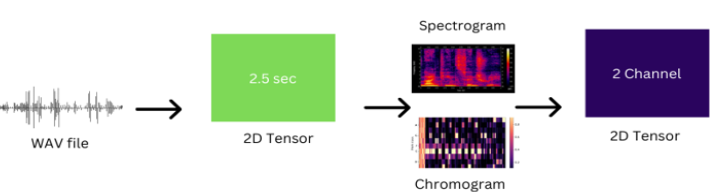
\includegraphics[scale=0.4]{Pre-Prrocessing.png}
Fig: Overview of the Preprocessing for Audio Data

\section{Convolutional Pipeline}
The convolutional pipeline begins by processing a 2-channel input tensor (e.g., spectrogram and chronogram) with dimensions \(2 \times 128 \times 64\). The first convolutional layer applies 24 filters of size \(5 \times 5\) with a stride of \(4 \times 2\) and no padding, reducing the spatial dimensions to \(24 \times 31 \times 30\). This layer is followed by batch normalization, which stabilizes feature maps, and a LeakyReLU activation with a slope of 0.01 to introduce non-linearity and mitigate the vanishing gradient problem. Next, a second convolutional layer applies 16 filters of size \(5 \times 5\) with a stride of \(1 \times 1\), further extracting complex features and producing an output size of \(16 \times 27 \times 26\). Similar to the first layer, batch normalization, and LeakyReLU activation is applied to ensure stable training and effective feature learning.

The pipeline then incorporates a max pooling layer with a kernel size of \(4 \times 2\) and stride \(4 \times 2\), down-sampling the feature maps to \(16 \times 6 \times 13\). A third convolutional layer applies 4 filters of size \(3 \times 3\) with a stride of \(1 \times 1\), extracting deeper hierarchical features and reducing the dimensions to \(4 \times 4 \times 11\). This is followed by batch normalization and LeakyReLU activation to maintain non-linearity and enhance learning. Finally, the output tensor is flattened into a 1D vector of size \(1 \times 176\), preparing it for downstream tasks such as classification or regression. This sequential architecture effectively reduces the input dimensions while capturing meaningful features for robust audio-based diagnostic predictions.
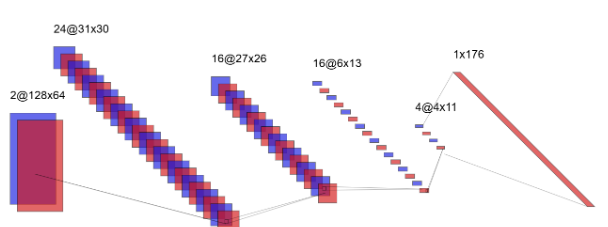
\includegraphics[scale=0.5]{Conv-Pipeline.png}
Fig: Overview of the Convolutional pipeline

\section{Combined Pipeline}

The combined pipeline integrates scalar and multidimensional inputs, processes them through a series of fully connected layers, and outputs predictions using a softmax function. The design is structured to progressively reduce dimensions while maintaining robust feature representation through non-linear activation and normalization techniques.

The scalar pipeline starts with a single linear layer that transforms a scalar input to the desired scalar output size. A LeakyReLU activation with a slope of 0.01 is applied to introduce non-linearity, enabling the network to capture complex relationships in the scalar input.

The combined pipeline begins by accepting the concatenated input vector which merges outputs from earlier stages. The first fully connected layer reduces the input to 1024 dimensions, followed by batch normalization to stabilize the training process and LeakyReLU activation for non-linearity. Dropout with a rate of 0.5 is applied to prevent overfitting. This pattern is repeated across four subsequent layers, progressively reducing dimensions from 1024 to 512, 128, 64, and finally the size of 8. At each stage, batch normalization and LeakyReLU activation enhance feature extraction, while dropout ensures robust generalization.

The final layer applies a softmax activation, converting the output into probabilities over the target classes. This combined pipeline effectively integrates scalar and multidimensional data, utilizing deep learning techniques to achieve accurate and interpretable predictions.
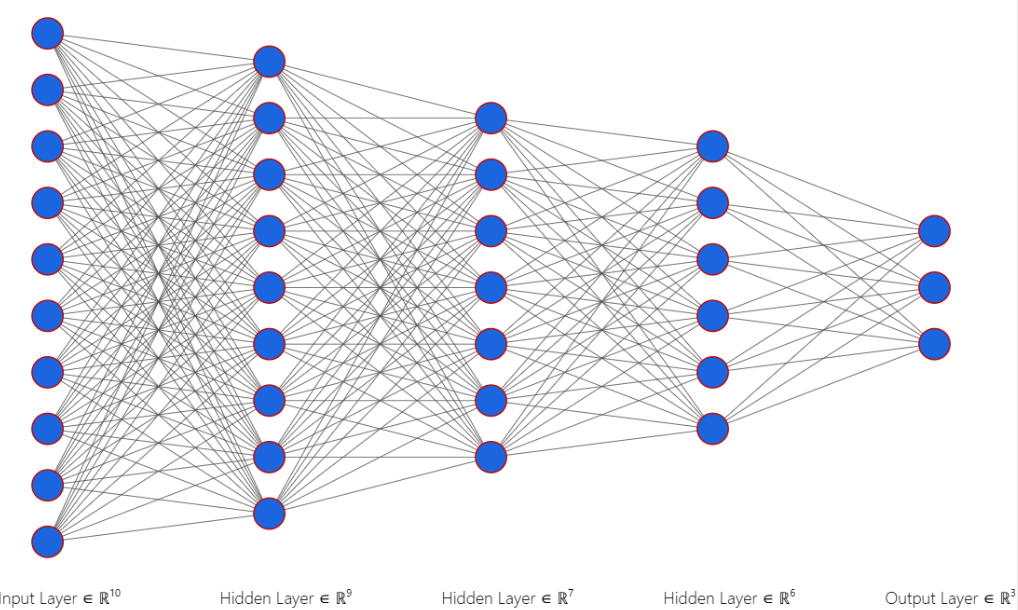
\includegraphics[scale=0.3]{Main Pipeline.png}
Fig: Overview of the Combined pipeline

\section{Model Evaluation}

The model achieved an overall accuracy of \(88.81\%\), correctly classifying 365 out of 411 test samples. This high accuracy indicates the model's strong ability to generalize across diverse diagnostic categories. The weighted precision of \(88.81\%\) shows the model's effectiveness in minimizing false positives, ensuring the majority of predicted classes are correct. Similarly, the weighted recall of \(88.81\%\) highlights the model's ability to identify actual positive cases accurately, demonstrating excellent sensitivity. The F1-score of \(88.81\%\), a balanced measure of precision and recall, further emphasizes the model's robustness and consistency.

From the class-wise analysis, categories like Asthma and Bronchiectasis exhibit strong correct prediction counts, with Asthma achieving a precision of approximately \(87.96\%\) and Bronchiectasis achieving high performance in both total and correct predictions. This consistency across major classes underlines the model's reliability. Furthermore, even for less frequent classes like Lung Fibrosis and Pleural Effusion, the model maintains stable prediction patterns, showing its ability to handle class imbalances. These results confirm the model's readiness for real-world diagnostic applications, supported by its high overall performance across metrics.
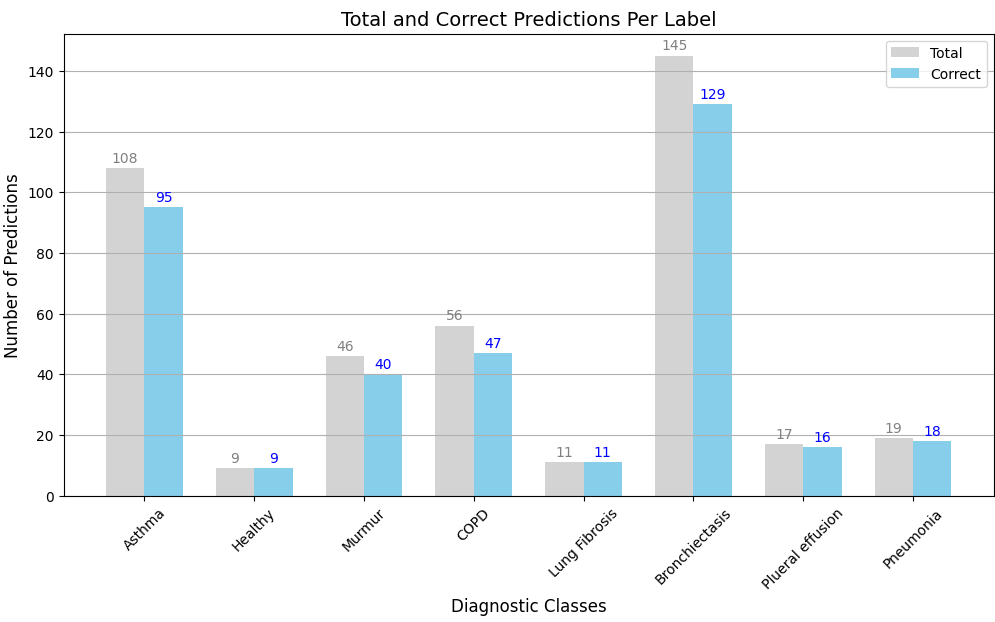
\includegraphics[scale=0.3]{Diagnostic.png}
Fig: Overview of Model Accuracy
\section{Conclusion}
yasmin to work on 


\begin{figure}[h]
  \centering
  \includegraphics[width=0.5\textwidth]{solar}
  \caption{Levelized cost of energy production by method of 
  generation. \cite{heart}}
  \label{fig:solar_cheap}
\end{figure}

\cite{telehealth}

\bibliographystyle{plain}
\bibliography{ESE_534_Report}

\appendix

\end{document}
\endinput
